\chapter{Предложение за алгоритми при обучение на изкуствени невронни мрежи}

\section{Бърз прототип на LibreOffice Calc с еволюция на разликите и оптимизация с рояк от частици}

Процесът по търсенето на оптимални тегла в изкуствена невронна мрежа от тип трислоен перцептрон много нагледно може да бъде демонстриран с бърз прототип в софтуерния пакет LibreOffice Calc. За осъществяване на прототипирането моделът на изкуствената невронна мрежа бива разгърнат в двузимерната равнина от клетки на електронната таблица. Търсенето на оптимални стойности за теглата в мрежата се постига чрез вградения в LibreOffice Calc модул за оптимизация наречен Solver (Фиг. \ref{fig001}).

\begin{figure}[h]
  \centering
  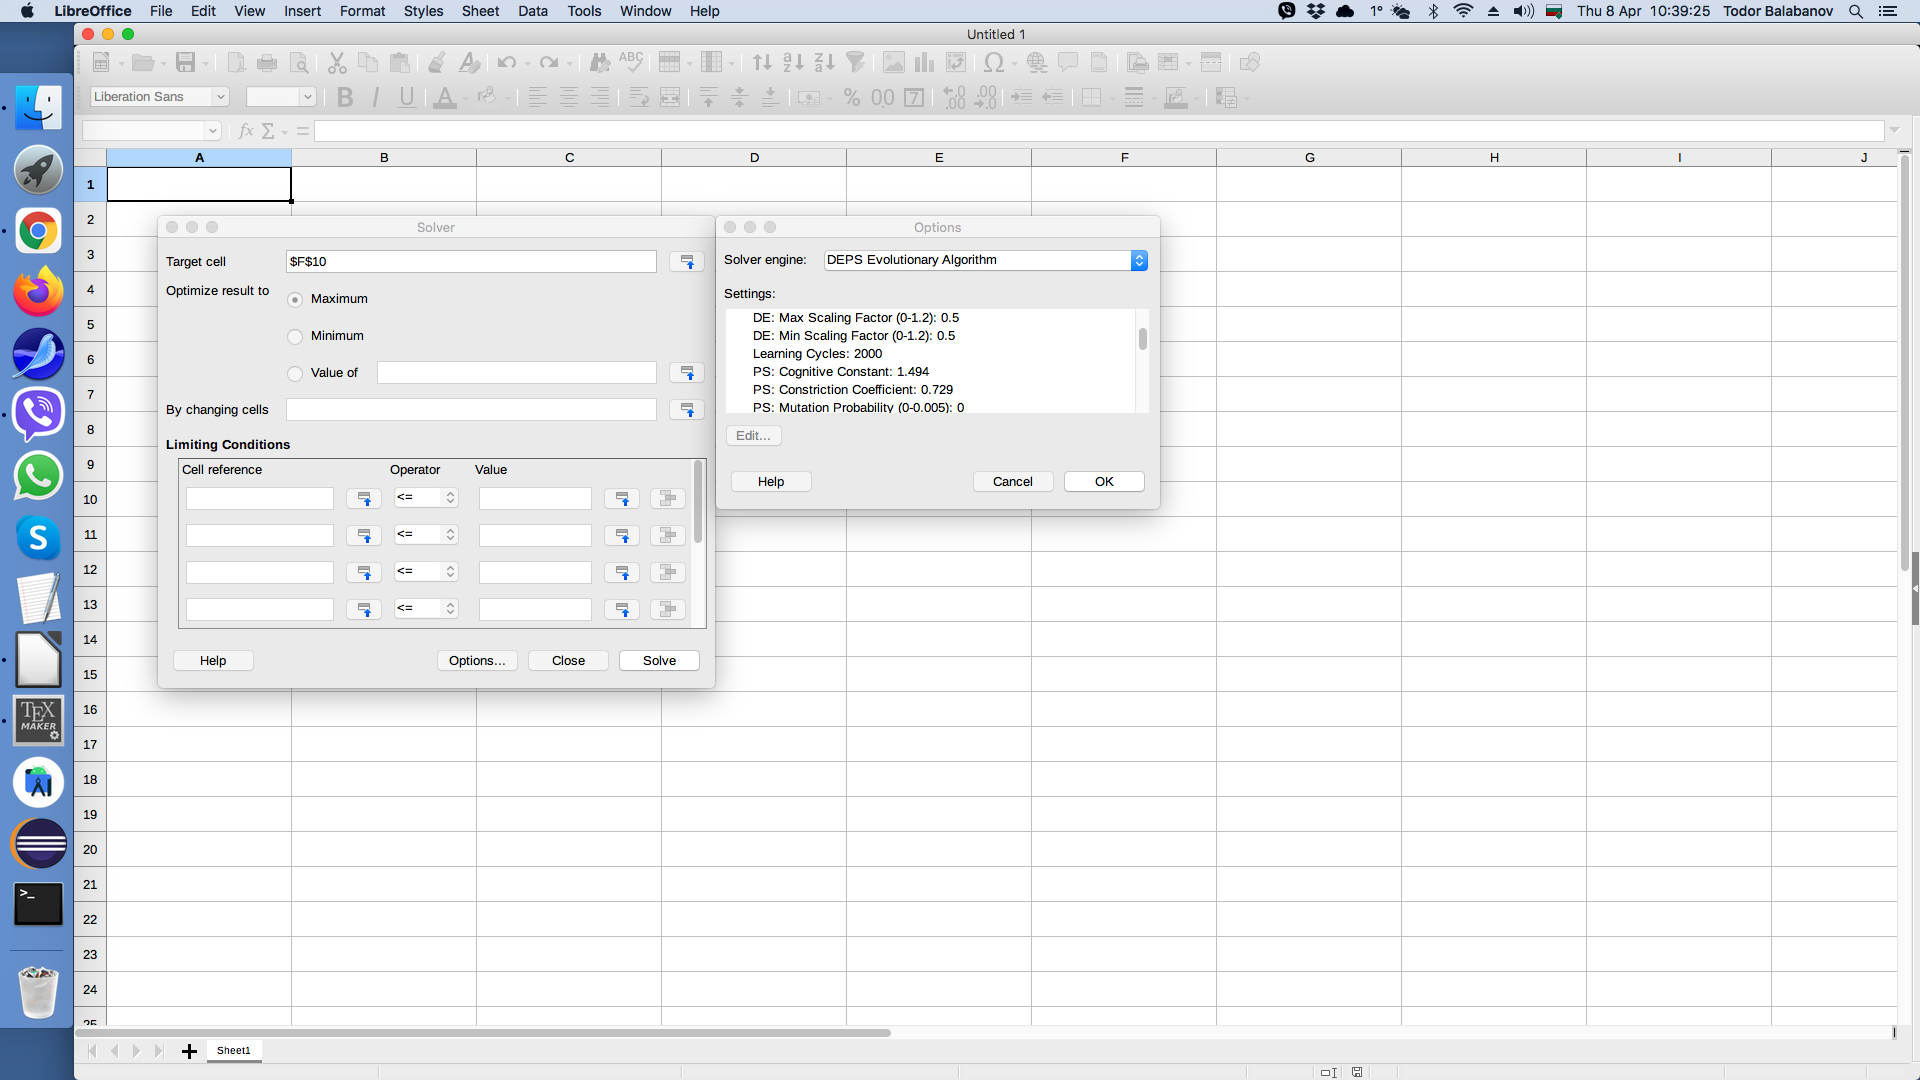
\includegraphics[width=1.0\linewidth]{fig001.png}
  \caption{Модул за оптимизация в LibreOffice Calc}
\label{fig001}
\end{figure}

За нелинейна оптимизация модулът прилага алгоритмите за еволюция на разликите и оптимизация с рояк от частици. Двата алгоритъма се прилагат в хибридна комбинация, като с предварително дефинирана вероятност е определено колко често ще бъде активиран всеки от тях. Модулът се настройва за клетка, чиято оптимална стойност ще бъде търсена (максимум, минимум или конкретно число). Също така, задава се и регионът от клетки, които подлежат на промяна в процеса по оптимизация. Като клетка в която ще се търси минимум при бързото протитипиране се избира общата средно-квадратична грешка допусната от изкуствената невронна мрежа. Регионът от клетки за оптимизация съдържа теглата използевани в изкуствената невронна мрежа. 

\begin{figure}[h]
  \centering
  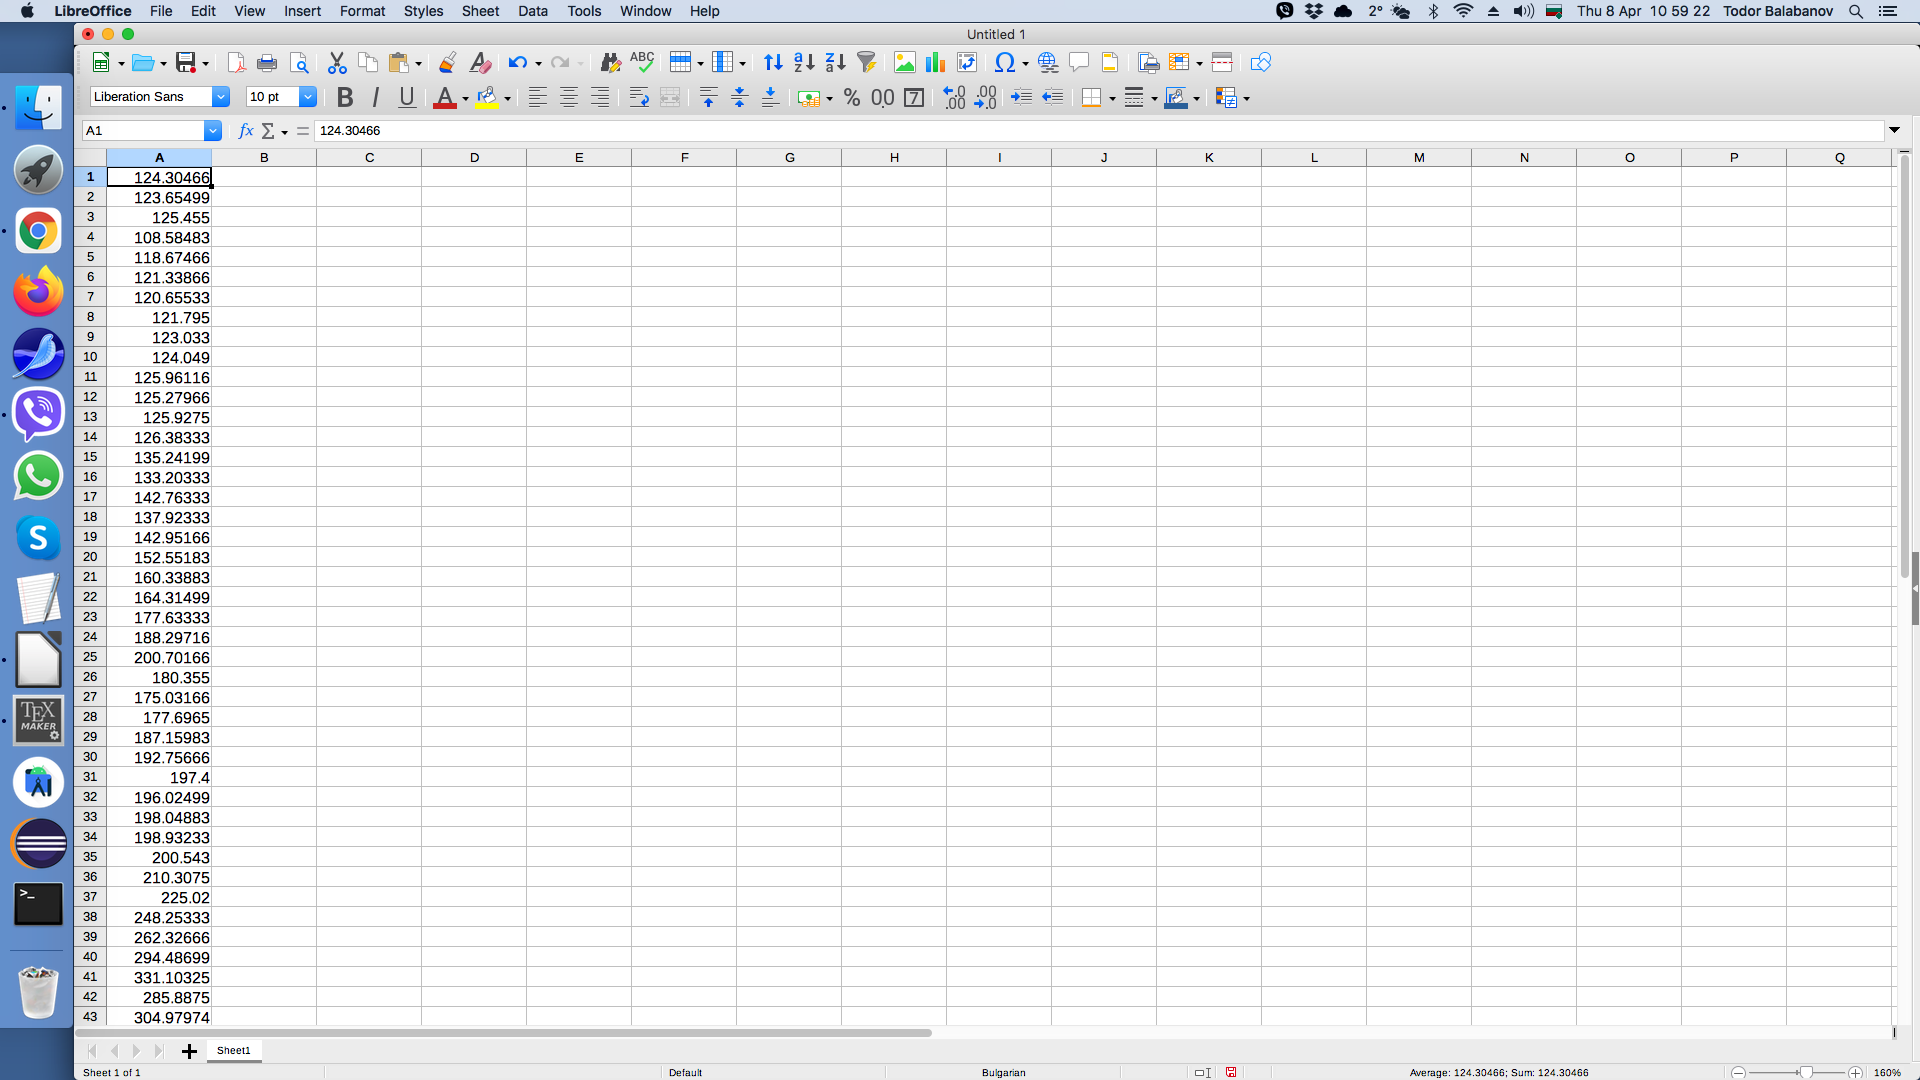
\includegraphics[width=1.0\linewidth]{fig002.png}
  \caption{Стойности на Bitcoin виртуалната валута}
\label{fig002}
\end{figure}

Като множество данни се използват стойностите на Bitcoin виртуалната валута (Фиг. \ref{fig002}), на дневна база, за няколко години назад. Моделът за прогнозиране се основава на нелинейна авторегресия. Това означава, че на входа на мрежата се подават мащабирани минали стойности от времевия ред, а на изхода на мрежата се очакват мащабирани прогнозни стойности. 

\begin{figure}[h]
  \centering
  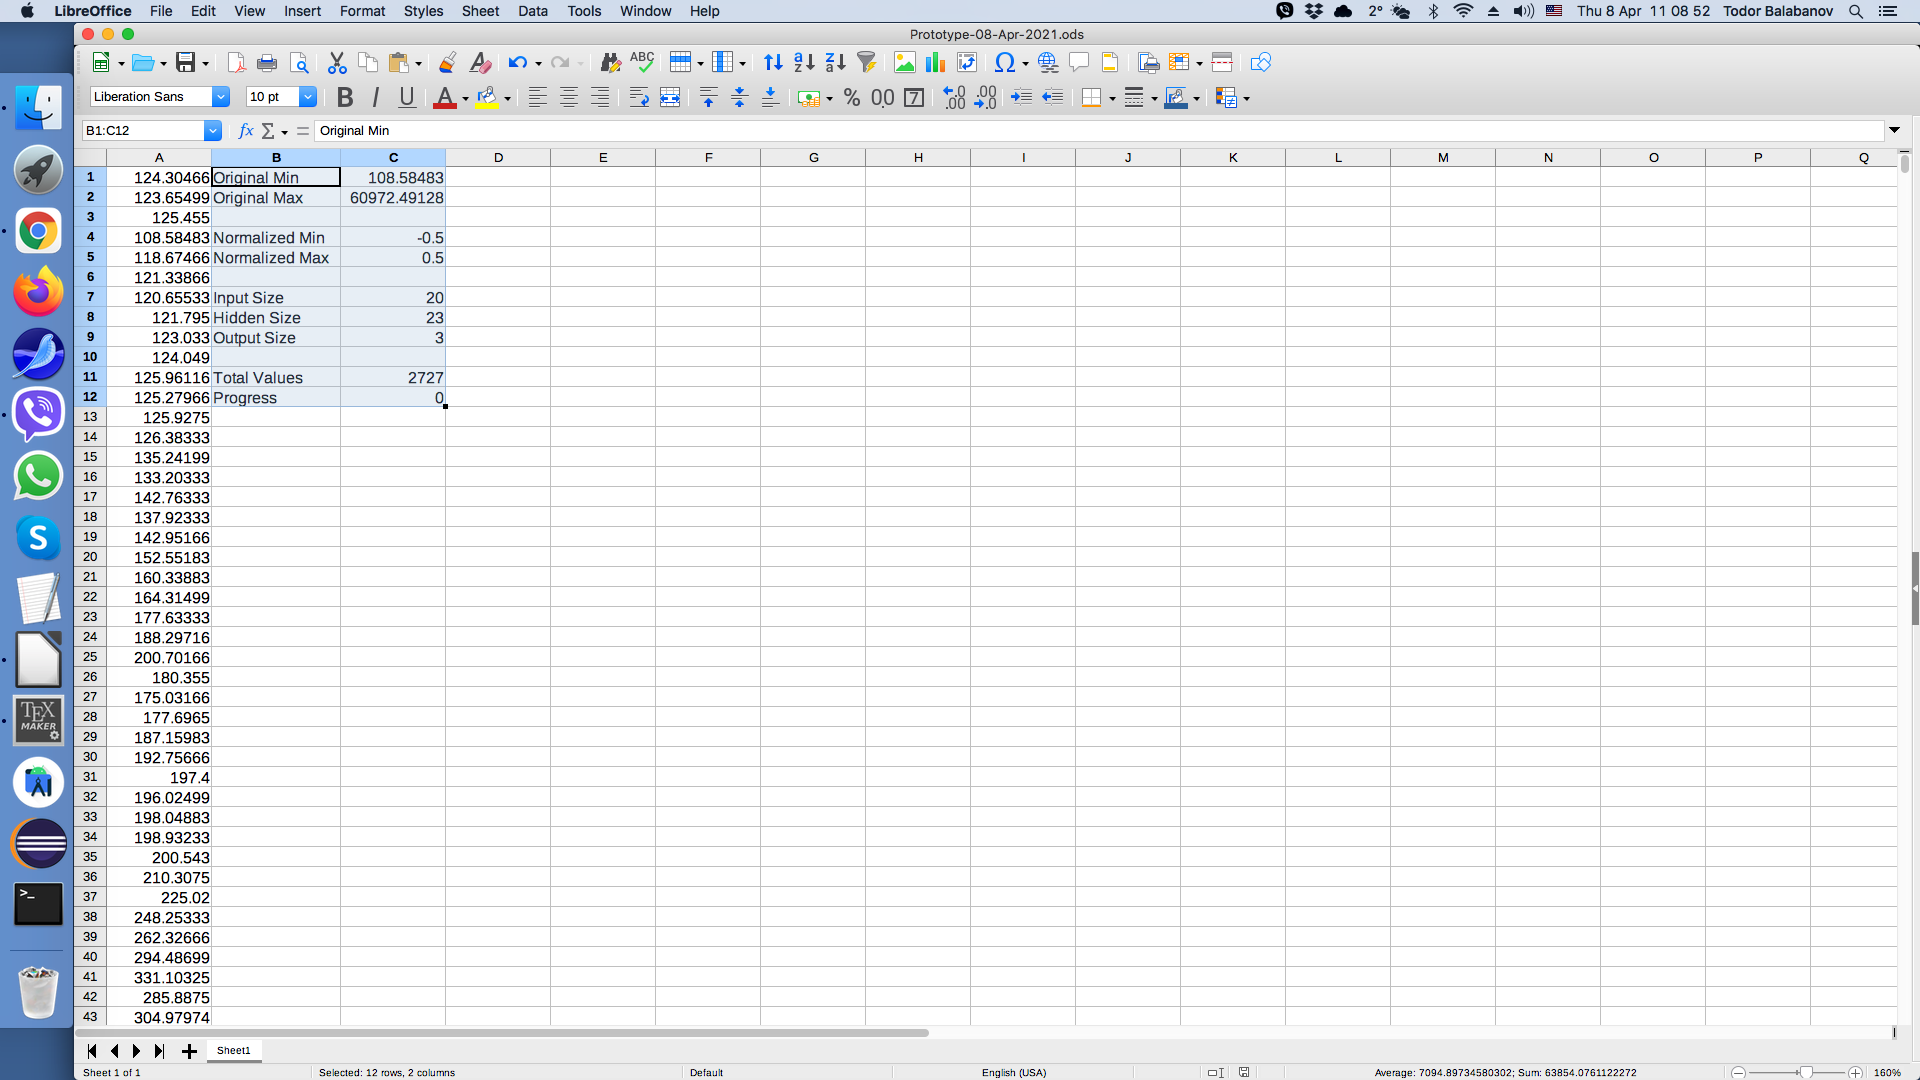
\includegraphics[width=1.0\linewidth]{fig003.png}
  \caption{Параметри на трислойната изкуствена невронна мрежа}
\label{fig003}
\end{figure}

След подбора на времеви ред следва избор на параметрите с които ще бъде напревен модела на трислойната изкуствена невронна мрежа (Фиг. \ref{fig003}). За целите на линейното мащабиране първо се намират най-малката и най-голямата стойност в оригиналния времеви ред, чрез формули в LibreOffice Calc: $=MIN(A:A)$ и $=MAX(A:A)$. Тъй като приложената прагова функция е хиперболичен тангенс, диапазона за мащабирания времеви ред е избран от -0.5 до +0.5. Умишлено се избягва мащабиране до асимптотичните стойности от -1.0 до +1.0, тъй като такова мащабиране много би увеличило стойностите на междинните пресмятания, а и не би дало възможност да се прогнозират по-малки или по-големи стойности от вече известните в оригиналния времеви ред. Топологията на мрежата се избира експериментално, като изходния слой има размер, според това колко стойности в бъдещето е желателно да се предсказват. Размера на входния слой се определя експериментално. За размера на скрития слой има различни емпирични правила, като най-популярното е скритият слой да бъде половината от сумата на размерите имащи входния и изходния слой. Съществуват адаптивни алгоритми, които чрез проби и грешки да определят топологията на мрежата, но в това бързо прототипиране тези алгоритми не се прилагат. 

Общият брой стойности в оригиналния времеви ред се определят с формула в LibreOffice Calc: $=COUNT(A:A)$. Тъй като процеса по „разгръщането“ на модела е относително бавен, то се добавя клетка в която да се проследява напредъка от Python скрипта в „разгръщането“. LibreOffice Calc позволява изпълнението на макроси, като се поддържат няколко програмни езика. Програмният език Python е изключително популярен в сферата на машинното самообучение и дава изключително големи възможности за частична автоматизация в програмите на LibreOffice.

След мащабирането на оригиналния времеви ред се формират тренировъчните примери, като за вход се вземат стойности преди условния момент $t_0$, а за очакван изход стойности след условния момент $t_0$ (условно разделяне на минало и бъдеще).

\begin{lstlisting}[caption=Мащабиране на оригиналния времеви ред, language=Python, basicstyle=\tiny, label=listing001]
    ''' Scale input. '''
    for t in range(1, total_values + 1):
        sheet.getCellRangeByName("E" + str(t)).setValue(sheet.getCellRangeByName("$C$4").getValue() + 
        (sheet.getCellRangeByName("$C$5").getValue() - sheet.getCellRangeByName("$C$4").getValue()) * ((sheet.getCellRangeByName("A" + str(t)).getValue() - 
        sheet.getCellRangeByName("$C$1").getValue()) / (sheet.getCellRangeByName("$C$2").getValue() - sheet.getCellRangeByName("$C$1").getValue())))
\end{lstlisting}

В листинг \ref{listing001} се демонстрира линейното мащабиране, като за извършване на изчисленията се използват установените минимални и максимални стойности (Фиг. \ref{fig004}). 

\begin{figure}[h]
  \centering
  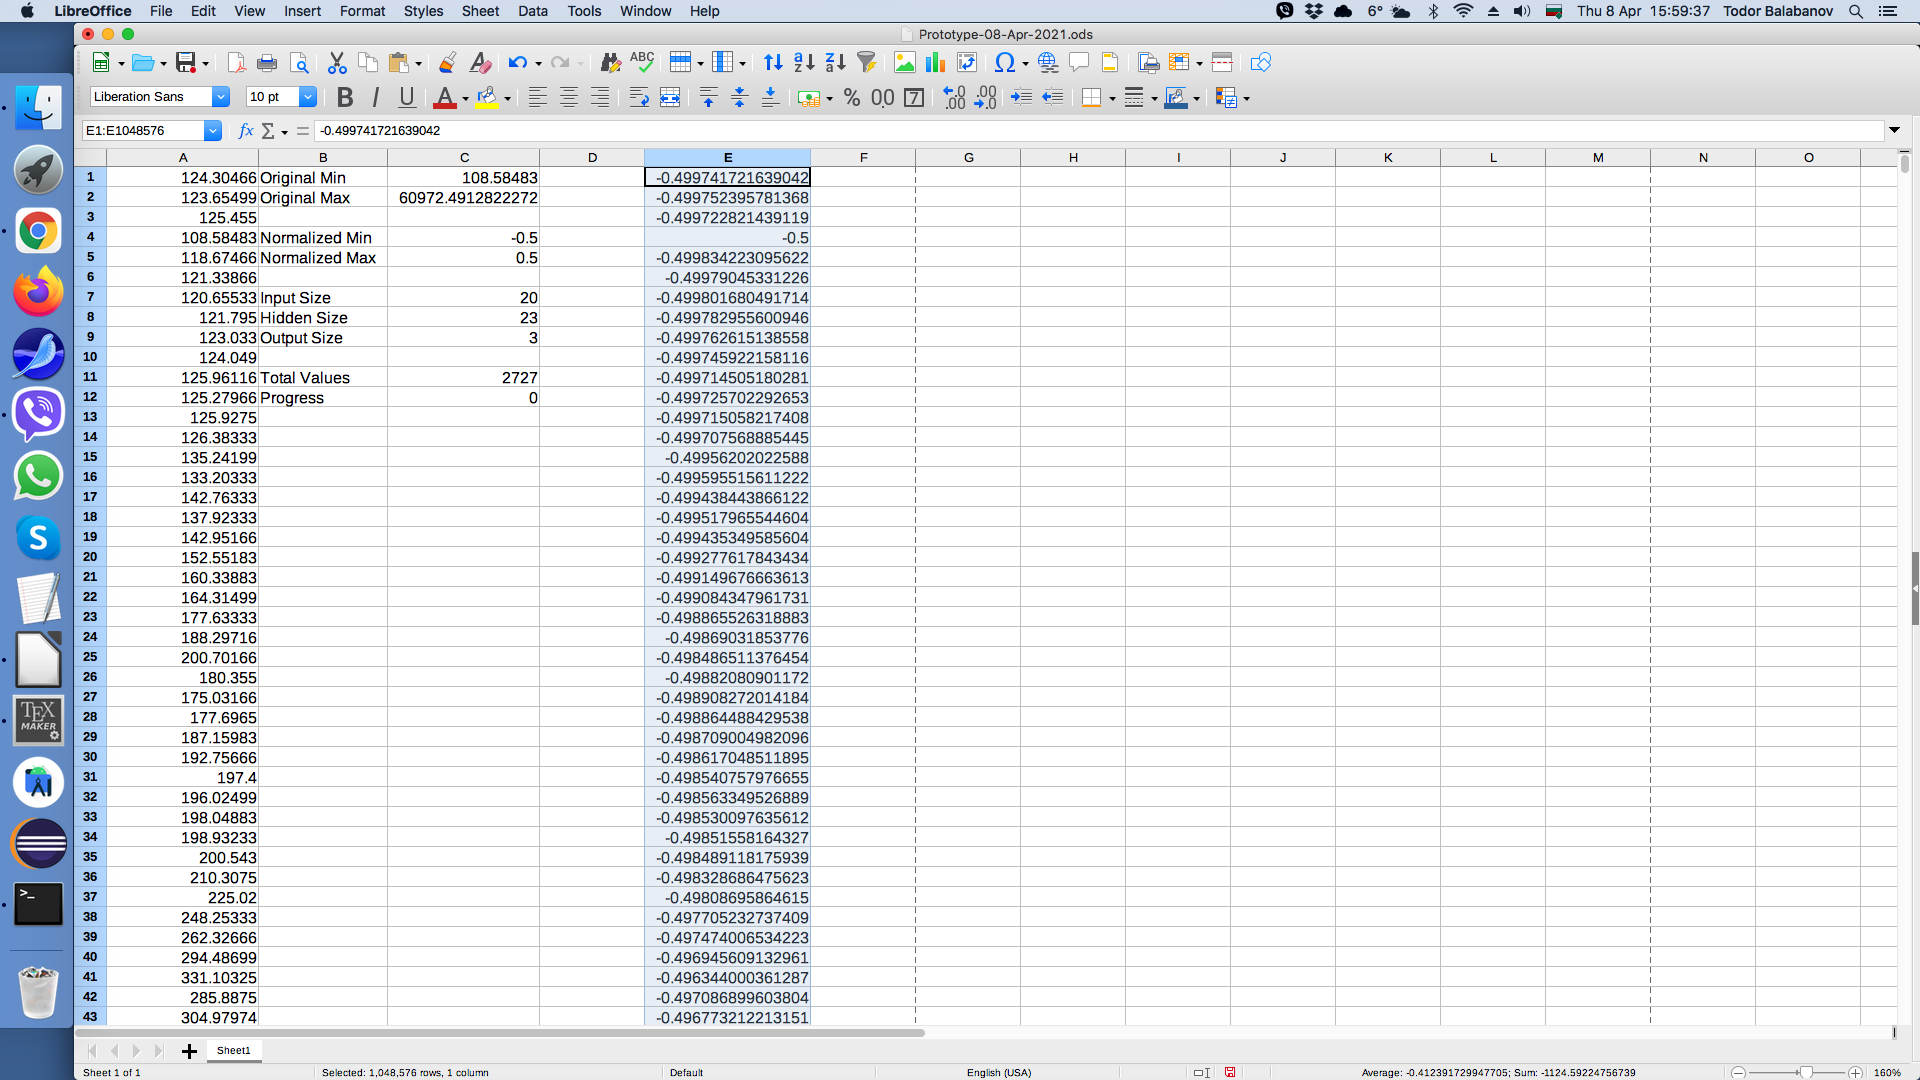
\includegraphics[width=1.0\linewidth]{fig004.png}
  \caption{Резултат от мащабирането на времевия ред}
\label{fig004}
\end{figure}

На всеки слой в изкуствената невронна мрежа се добавя по един допълнителен неврон (Листинг \ref{listing002}), постоянно емитиращ единична стойност (отместване или от английски език bias).

\begin{lstlisting}[caption=Неврони емитиращи постоянно единичен сигнал, language=Python, basicstyle=\tiny, label=listing002]
        ''' Setup biases. '''
        sheet.getCellRangeByName("G" + str(x)).setValue(1)
        sheet.getCellRangeByName("G" + str(x)).CellBackColor = (255 << 16 | 255 << 8 | 0)
        sheet.getCellRangeByName("H" + str(x)).setValue(1)
        sheet.getCellRangeByName("H" + str(x)).CellBackColor = (255 << 16 | 255 << 8 | 0)
        sheet.getCellRangeByName("I" + str(x)).setValue(1)
        sheet.getCellRangeByName("I" + str(x)).CellBackColor = (255 << 16 | 255 << 8 | 0)
        sheet.getCellRangeByName("J" + str(x)).setValue(1)
        sheet.getCellRangeByName("J" + str(x)).CellBackColor = (255 << 16 | 255 << 8 | 0)
\end{lstlisting}

Мащабираният времеви ред бива „разбит“ условно на „минали“ стойности и „бъдещи“ стойности. Миналите стойности стават входни сигнали за изкуствената невронна мрежа (Листинг \ref{listing003}).

\begin{lstlisting}[caption=Формиране на входния слой, language=Python, basicstyle=\tiny, label=listing003]
        ''' Input data loading. '''
        for i in range(1, input_size + 1):
            sheet.getCellRangeByName("G" + str(x + i)).setValue(sheet.getCellRangeByName("E" + str(t + i)).getValue())
            sheet.getCellRangeByName("G" + str(x + i)).CellBackColor = (255 << 16 | 0 << 8 | 0)
\end{lstlisting}

По аналогичен начин, будещите стойности се зареждат като очакван изход от изкуствената невронна мрежа (Листинг \ref{listing004}).

\begin{lstlisting}[caption=Очакван изход от мрежата, language=Python, basicstyle=\tiny, label=listing004]
        ''' Expected data loading. '''
        for e in range(1, output_size + 1):
            sheet.getCellRangeByName("J" + str(x + e)).setValue(sheet.getCellRangeByName("E" + str(t + e + input_size)).getValue())
            sheet.getCellRangeByName("J" + str(x + e)).CellBackColor = (0 << 16 | 127 << 8 | 0)
\end{lstlisting}

Стойностите във възлите на скрития слой са резултат от пресмятане на входните сигнали и текущите стойности на теглата в мрежата (Листинг \ref{listing005}). 

\begin{lstlisting}[caption=Стойности на скрития слой при правия пас, language=Python, basicstyle=\tiny, label=listing005]
        ''' Setup hidden layer. '''
        wih = 1
        for h in range(1, hidden_size + 1):
            sum = ""
            for i in range(0, input_size + 1):
                sum = sum + "G" + str(x + i) + "*Q" + str(wih)
                wih = wih + 1
                if i < input_size:
                    sum = sum + " + "
            sheet.getCellRangeByName("H" + str(x + h)).setFormula("=TANH( " + sum + " )")
            sheet.getCellRangeByName("H" + str(x + h)).CellBackColor = (0 << 16 | 0 << 8 | 255)
\end{lstlisting}

На свой ред, стойностите в изходния слой са резултат от пресмятане на сигналите в скрития слой и текущите стойности на теглата в мрежата (Листинг \ref{listing006}).

\begin{lstlisting}[caption=Стойности на изходния слой при правия пас, language=Python, basicstyle=\tiny, label=listing006]
        ''' Setup output layer. '''
        who = 1
        for o in range(1, output_size + 1):
            sum = ""
            for h in range(0, hidden_size + 1):
                sum = sum + "H" + str(x + h) + "*S" + str(who)
                who = who + 1
                if h < hidden_size:
                    sum = sum + " + "
            sheet.getCellRangeByName("I" + str(x + o)).setFormula("=TANH( " + sum + " )")
            sheet.getCellRangeByName("I" + str(x + o)).CellBackColor = (0 << 16 | 255 << 8 | 0)
\end{lstlisting}

Стойностите в изходния слой, спрямо очакваните стойности дават грешката, която изкуствената невронна мрежа допуска за конкретния тренировъчен пример (Листинг \ref{listing007}).

\begin{lstlisting}[caption=Стойност на грешката допусната от мрежата за конкретния пример, language=Python, basicstyle=\tiny, label=listing007]
        ''' Network output error. '''
        for r in range(1, output_size + 1):
            sheet.getCellRangeByName("K" + str(x + r)).setFormula("= (J" + str(x + r) + "-I" + str(x + r) + ") * (J" + str(x + r) + "-I" + str(x + r) + ")")
            sheet.getCellRangeByName("K" + str(x + r)).CellBackColor = (0 << 16 | 255 << 8 | 255)
\end{lstlisting}

Така описаното разполагане по клетките на листа в електронната таблица се повтаря многократно, така че да се появи фрагмент за всеки тренировъчен пример. Фрагментът съдържа входен слой, скрит слой, изходен слой и очаквани на изхода стойности (Фиг. \ref{fig005}).

\begin{figure}[h]
  \centering
  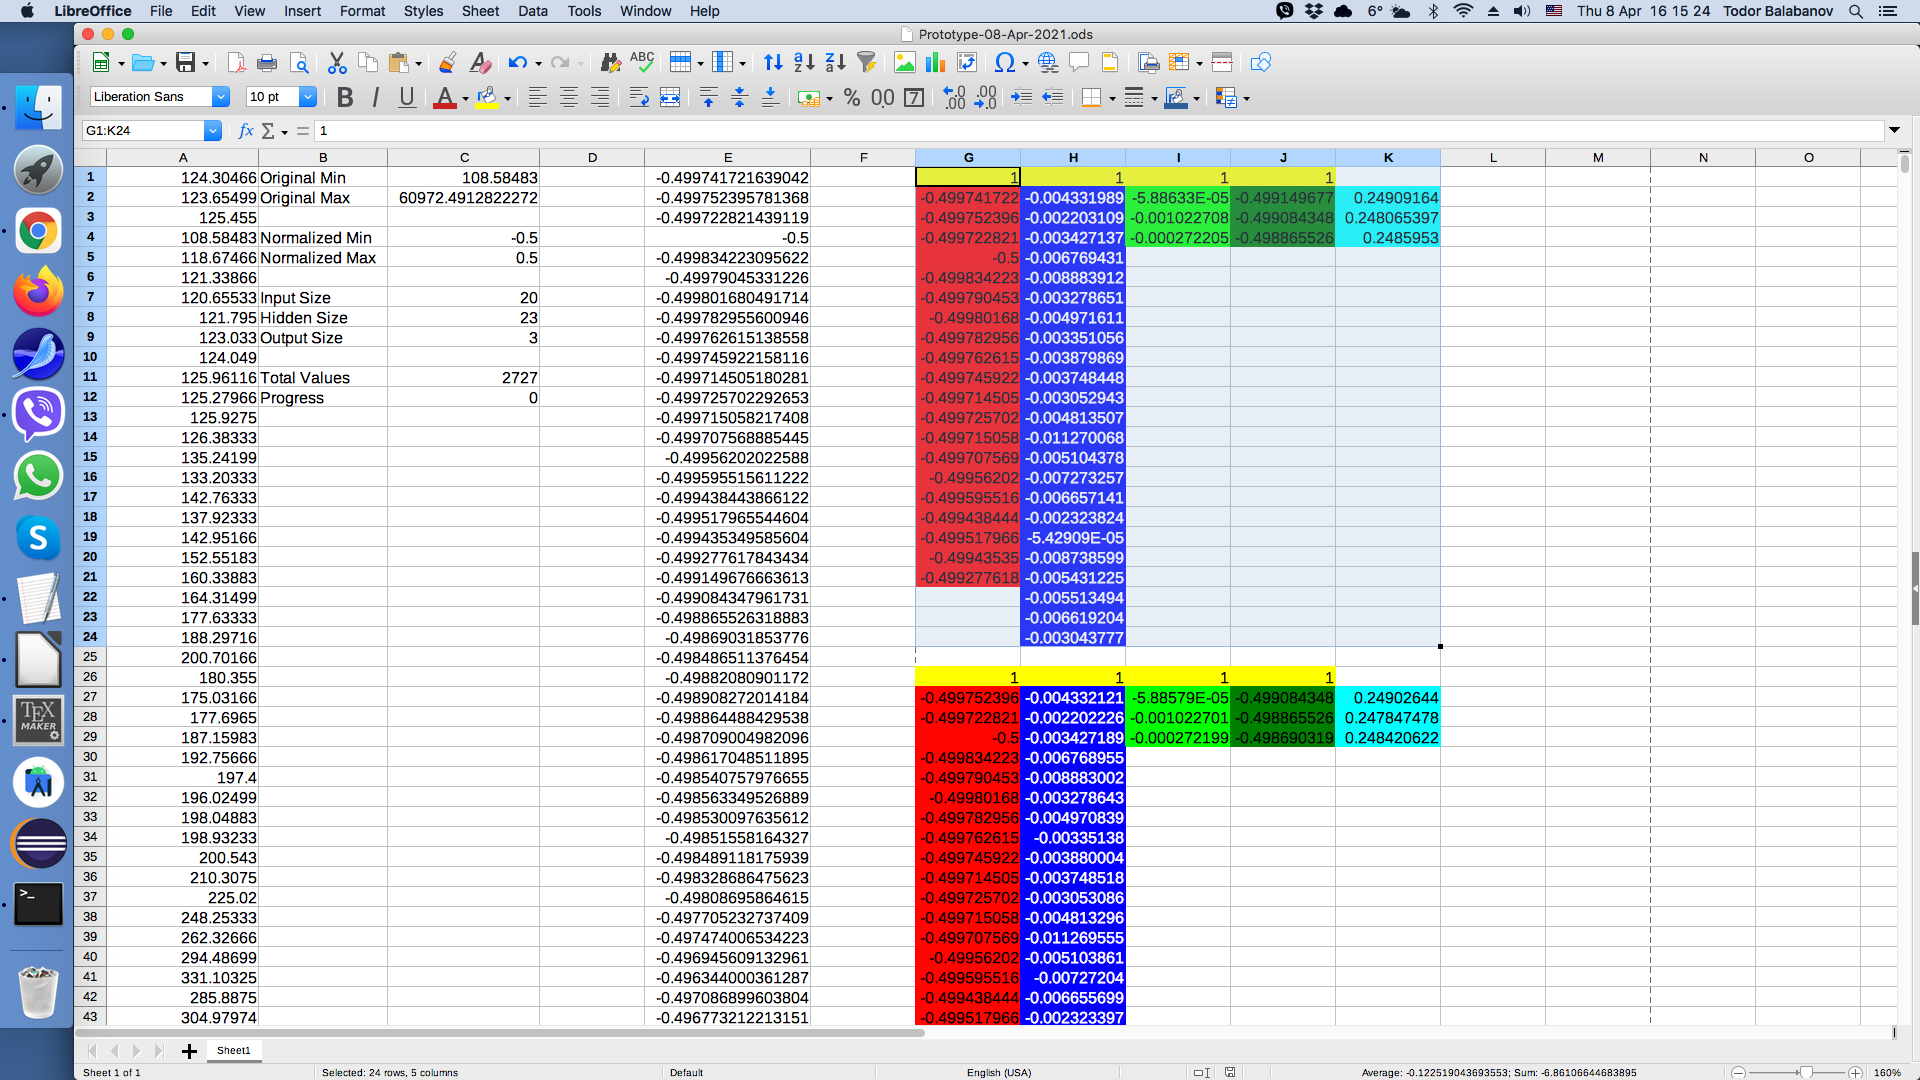
\includegraphics[width=1.0\linewidth]{fig005.png}
  \caption{Фрагменти за тренировъчните примери}
\label{fig005}
\end{figure}




